\section{Dataset and Marker Set}
One of the vital stages in research is building a pertinent dataset.
The dataset's quality can profoundly influence research outcomes. Here, we detail the technological methodology used to collect the dataset and its constituents.
Our main goal is an automated method to identify the start of full-body human movement and determine the most effective predictive movement feature.
To achieve this, we aim to curate a dataset that supports these goals.
Central to this research is capturing motion dynamics accurately.
Thus, we require technology for efficient bodily movement capture, like the Motion Capture System (MoCap).
This dataset is meticulously compiled with skilled dancers' valuable contribution.
Their expertise shapes the dataset, capturing precise and clear movements.
The dancers' involvement is crucial, as their understanding of body mechanics results in cleaner motion data.
This collaboration yields expressive movements with distinct starting points, aligning with research goals.
Their expertise elevates dataset quality, providing a resource that encapsulates human motion intricacies accurately and artistically.


\subsection{Dataset}
The dataset contains two categories of expressive movements, each associated with a different recording session. \\
The details of both types of movements are provided below.
The dataset comprises <NUMERO FINALE FRAMMENTI> segments recorded using the \textit{Qualisys Motion Capture system}.
These segments represents various subjects performing simple movement sequences, which are captured from different angles using some cameras.
The videos are synchronized through SMPTE timecode and each video is accompanied by corresponding motion capture data that records the positions of body parts.


\subsubsection{Wholodance Dataset}
\subsubsection{Montpellier - UniGe Dataset}

\subsection{Dataset Validation with Cohen's Kappa}
Each fragment of the dataset was classified by us, the thesis students, our professors, and the expert dancer Cora Gasparotti, identifying one or more connections between two joints responsible for the origin of the movement in question.
To measure agreement between validators, we used the Cohen's Kappa $\kappa$, a statistical coefficient commonly used to assess reliability or concordance among human observers or automated systems in the categorization process.
It is generally thought to be a more robust measure than simple percent agreement calculation, as $\kappa$ takes into account the possibility of the agreement occurring by chance.



\subsection{Full Marker Set}

\begin{figure}[H]
    \centering
    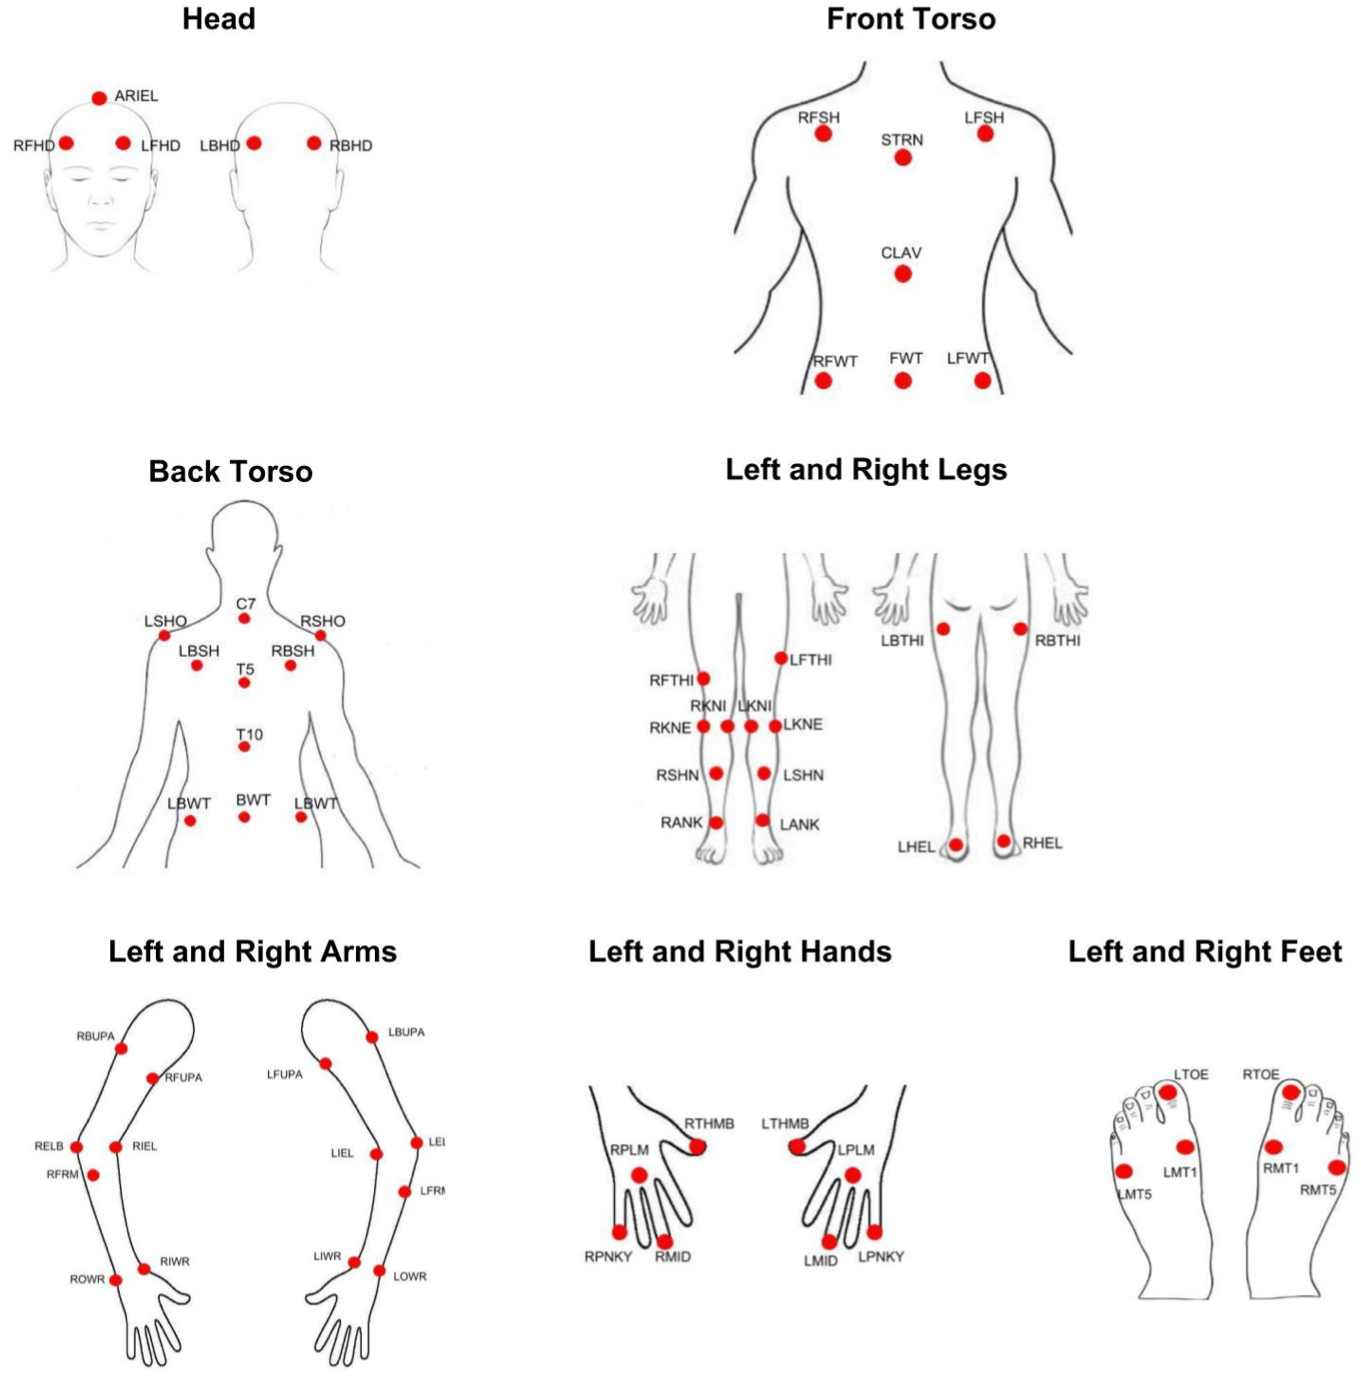
\includegraphics[width=0.9\textwidth]{graphics/full_marker_set.png}
    \caption{Full Marker Set of 64 markers}
    \label{fig:full_marker_set}
\end{figure}


\subsection{Reduced Marker Set}
The reduced marker set is achieved by reducing the count of markers employed from the full marker set.
This because a simplified skeletal framework can adeptly communicate essential insights about expressive movements.
The reduction of multiple markers into individual joints is implemented to mitigate the possibility of marker omission.
This reduction was performed by computing the $barycentre$ of joints in a cluster as follows:
\begin{enumerate}
    \item Extract the $x$, $y$, $z$ $coordinates$ for each marker of the cluster.
    \item Compute for each of $x$, $y$, $z$ their average, by summing all the $x$-markers together
    (and similarly for $y$ and $z$) and then dividing by the number of markers in the cluster.
\end{enumerate}    

\begin{table}[H]
    \centering
    \begin{tabular}{|c|c|}
        \hline
        \textbf{Reduced Marker Set Labels} & \textbf{Full Marker Set Labels} \\
        \hline
        right\_foot & RHEL, RMT10, RMT5 \\
        left\_foot & LHEL, LMT10, LMT5 \\
        right\_ankle & RANK \\
        left\_ankle & LANK \\
        right\_knee & RKNE, RKNI \\
        left\_knee & LKNE, LKNI \\
        right\_hip & RFWT, RBWT \\
        hip\_centre & RFWT, LFWT, RBWT, LBWT \\
        left\_hip & LFWT, LBWT \\
        spine & C6, T5, T10, BWT \\
        right\_hand & RPLM, RTHMB, RMID, RPNKY\\
        left\_hand & LPLM, LTHMB, LMID, LPNKY \\
        right\_wrist & ROWR, RIWR \\
        left\_wrist & LOWR, LIWR \\
        right\_elbow & RELB, RIEL\\
        left\_elbow & LELB, LIEL \\
        right\_shoulder & RSHO \\
        shoulder\_centre & LSHO, RSHO \\
        left\_shoulder & LSHO \\
        head & RBHD, LBHD, LFHD, RFHD, ARIEL \\
        \hline
    \end{tabular}
    \caption{Mapping of the full marker set to the reduced marker set}
    \label{tab:labels_joints}
\end{table}


